\chapter{基于弱监督注意力的多人姿态估计方法}
\label{cha:method}

\section{概述}
\label{sec:methodoverview}
%   This part intends to state the overall idea
本方法使用基于残差网络\footnote{残差网络,简称ResNet, 全称Residual Network}与特征金字塔网络\footnote{特征金字塔网络,简称FPN, 全程Feature Pyramid Network}结构的网络框架作为特征提取的骨架,为模型提供各个尺度的特征图。在特征提取部分之后,网络可以分为目标检测与姿态估计和融合回归两个步骤。在目标检测与姿态估计过程中,网络预测出目标的边界框,粗略的关键点预测和实例分割结果。而在融合回归部分,网络会接受从目标检测与姿态估计阶段产生的结果并将它们一同以一定的方式互相交汇并一起回归。而且,在融合回归的过程中,网络采取了多阶段的堆叠和中继监督的策略来共同精炼关键点与实例分割的结果。这种结构是受到CPM\cite{wei2016convolutional}的启发而设计的。同时,为了有效地融合实例分割与姿态估计的结果,网络使用了注意力机制,使其根据实例分割的生成注意力关注网络对应的区域,从而达到方法最初设计的目的,也就是解决多人检测下姿态遮挡的问题。同时,考虑到姿态估计的信息对实例分割也有促进作用,我们设计了双流的网络结构让模型在每个阶段都能同时预测分割结果和姿态估计结果,并送入下一阶段继续优化。网络的整体结果如图\ref{fig:Overall}

%	ROI Extraction
%	key-point & Mask Prdiction
%		Stage One's Prediction
网络通过特征提取器$E$得到图像$I$来自网络各个尺度的特征$F=\{f_1, f_2, ..., f_5\}$。这些特征被兴趣区域对齐层\footnote{兴趣区域对齐层,简称RoI Align Layer, 全称Region of Interest Align Layer}通过双线性插值的方法调整到了同样的尺寸。每个图像中只有来自特定尺度$k$的特征图$f_k$被选中并被输入至接下来的目标检测与姿态估计部分。这个被选中的特征被分别送入了目标检测分支$D$与姿态估计分支$P$,分别得到了实例分割结果$S_1=\{s_1^1, s_1^2, ..., s_1^n\}$与姿态估计结果$K_1=\{k_1^1, k_2^1, ..., k_1^n\}$。这些中间结果会被输入到融合优化阶段进行多阶段的回归。

\begin{figure*}[htbp]	
	\centering
	\includegraphics[scale=0.4]{network.eps}
	\caption{网络整体结构}
	\label{fig:Overall}
\end{figure*}

%		Stage 2+'s Prediction
如图\ref{fig:RefineNet}所示,在融合优化阶段的第$t(t>2)$阶段,单个优化模块接收来自特征提取器$E$的特征$f_k$、在阶段$t-1$中得到的姿态估计结果$K_{t-1}$与实例分割结果$S_{t-1}$。整个网络有主要设计亮点可以归纳为三点。第一是我们引入了注意力机制让网络关注具体的区域,我们设计了注意力转换模块来让生成一个合适的注意力与特征图融合,最后得到关键点预测结果$K_t$。第二,网络还会根据姿态估计的中间结果,也就是一些更偏向于得到关键点预测的特征,生成实例分割的结果。这让网络会根据来自姿态估计的信息修正实例分割的结果。最后,由注意力转换模块生成的注意力还会与从姿态估计那一支生成的中间结果融合,最终生成的实例分割的优化结果$S_t$。因此,整个优化模块$R$可以被抽象为形如公式\eqref{def:refinenet}的函数。


\begin{equation}
\label{def:refinenet}
M_t, K_t = R(M_{t-1}, K_{t-1})
\end{equation}

%   This part is to describe why we use a hybrid multi-stage arch
%	1. mask and key-point detection is associated
%	2. In crowd, the heatmap is not robust to predict
本方法使用了多阶段、利用弱监督约束的注意力的结构,同时优化实例分割与姿态估计的结果。首先多阶段与中继监督这两个设计可以让网络获得更大的感受野,让网络能够充分学习关键点之间的关系\cite{wei2016convolutional}。其次,由于实例分割和姿态估计是联系紧密的两个任务, 正如本文\ref{sec:generalmotivation}中提到的,实例分割与姿态估计能够相互优化,并且有相当大的相关性。所以这样设计的结构主要是希望能够同时优化姿态估计与实例分割结果。通过引入注意力以及弱监督这种较宽松约束下的可学习参数,网络能够更加适应数据中的不同表现。这让网络在一些实例分割无法正确引导关键点检测的情况下, 仍然能够生成较为正确的注意力引导关键点的检测与人体骨架的重建。

\begin{figure*}[htbp]	
	\centering
	\includegraphics[scale=0.65]{RefineNet.pdf}
	\caption{融合优化模块具体设计}
	\label{fig:RefineNet}
\end{figure*}

\section{目标检测与姿态估计}
\label{sec:detectionstage}
%	Structure description
%	1. Hybrid arch of maskrcnn & cpm
本文在特征提取部分使用了101层的残差网络与特征金字塔网络来生成不同尺度的特征图供检测部分使用。正如Mask R-CNN\cite{He2017Mask}中使用的结构,本文也设计了并行的区域建议网络,在经过回归分支后从不同尺度的特征图上得到来自不同尺度的边界框。这些尺度不同的边界框会根据其来源送入专为特征金字塔网络设计的兴趣区域对齐层,根据公式选定对应的层数来裁剪并对齐特征图\cite{Lin2016Feature}。这样裁剪下来的特征图具有相对平衡的感受野:小尺寸物体有较小的感受野大小,同时大尺寸物体会获得更大的感受野大小。

检测部分是由两个并行的分支组成的。实例分割与姿态估计分支分别使用裁剪好的特征得到粗略的实例分割结果与姿态估计结果。分割分支的网络结构使用了四层卷积核大小为3像素的卷积层,和一层步长为2,卷积核大小为2的空洞卷积层。同样的,姿态估计分支使用了五层卷积核大小为3的卷积层,最终的输出被两层1x1卷积调整至关键点外加背景个通道,以得到每个关键点的热力图。


%   Training strategy description
%	Section 1
在检测部分的监督过程中,由于我们将网络设计为能够完成两个任务的并行的分支,所以该部分的损失函数设计就表现为两个损失函数加和的形式。首先我们需要对目标位置检测进行监督,所以我们就借鉴区域卷积神经网络\cite{Girshick_2014_CVPR}中损失函数设计思路,使用交叉熵来计算预测标签与真实标签之间的距离。同样的,如Mask R-CNN\cite{He2017Mask}中的损失函数设计,交叉熵也被用来监督实例分割。
     

\section{融合优化}
\label{sec:refine}
\subsection{网络结构}
\label{subsec:architecture}
%	TODO: more detailed content to discuss the net structure in refine section
%	1. What the network looks like
%	2. Why we propose the network like this? (need to be explain by experiments)
%		a) training process (featured points)
%			(i)		loss penalty calculation
%		b) inference process 
%			(i)		attention-like instance segmentation
%Size of reception field is crucial to the refine section, as the key-point branch need them to avoiding the wrong decision in 
融合优化阶段由数个完全一样的优化模块组成,每个模块可以被抽象地定义为公式\eqref{def:refinenet}。首先,优化模块会把输入的特征分为两部分。第一份拷贝$f$会首先与来自阶段$t-1$的姿态结果$K_{t-1}$进行合并,并一同被送入一组共享的卷积层$C$中,得到姿态特征图$c$,如公式\eqref{def:sharedconv}\footnote{公式中的$\otimes$代表张量连接操作。}。第二份特征图拷贝$f$同样会与上一阶段的实例分割结果$S_{t-1}$进行合并,并被输入至注意力转换模块$A$中,得到注意力特征图$a$,如公式\eqref{def:attenconverter}\footnote{公式中的$\odot$代表张量内积操作。}。像公式\eqref{def:keypointhead}所描述,之后姿态特征图$c$会与经过$\sigma$门\footnote{$\sigma$门由一组神经层和一个$sigmoid$激活函数组成,会将网络输出限制在$[0,1]$的值域中}重新映射的注意力$a_s$相乘,经过姿态子网$H_k$的调整,最终输出关键点预测结果$K_t$。这样的设计让网络能够根据实例分割的结果生成注意力,让网络根据生成的注意力$a$生成更加鲜明的姿态估计结果。

\begin{equation}
\label{def:sharedconv}
c = C(f\otimes{K_{t-1}})
\end{equation}
\begin{equation}
\label{def:attenconverter}
a = A(f\otimes{M_{t-1}})
\end{equation}
\begin{equation}
\label{def:keypointhead}
K_t = H_k(c\odot \sigma(a))
\end{equation}

由注意力转换模块生成的注意力特征图$a$,不光会影响关键点预测的结果$K_t$,还会影响实例分割的结果$S_t$。如公式\eqref{def:fusion}所示,首先网络会利用来自共享卷积层的姿态特征图$c$生成一组供实例分割使用的特征图。这组特征图接下来会与经过$\tanh$门\footnote{$\tanh$门由一组神经层和一个$\tanh$激活函数组成,会将网络输出限制在$[-1, 1]$的值域中。}调整的注意力$a_t$相加,融合了来自注意力转换模块的信息,共同送入分割子网$H_s$得到最终优化的分割结果$S_t$。

\begin{equation}
\label{def:fusion}
S_t = H_s(F(c) \oplus \tanh(a))
\end{equation}

本文在选取注意力的表现形式时,使用了软注意力作为交替优化中媒介。实际上,实例分割的结果可以被当做一种注意力。因为使用分割结果在网络后处理阶段直接进行点乘处理,也就是在关键点热图使用分割结果做遮罩操作,在简单的融合实例分割信息的多人姿态估计策略中是很常见的。这种处理就相当于强化了对应空间位置的热图相应,也就是与注意力的机理是相似的。虽然实例分割也是网络自生成的结果,但由于其并不能完全满足多人姿态估计的要求,那么单独设计的使用实例分割信息监督影响的注意力就显得非常重要了。另外,实例分割结果是二值化图像,相当于一种硬注意力。与软注意力相比,硬注意会直接消除特征图对应位置的特征相应,损失了很多网络预测关键点位置所依赖的特征。并且这样使用硬注意力的系统会受限制于硬注意力本身,一旦生成的硬注意力不准确,就会在像姿态估计这种对于精确度要求很高的任务上失败。这说明软注意力在完成任务的目标上是必须的。

本文提出的优化模块主要可以让两个任务互相交替优化:第一,姿态估计会想实例分割提供特征图,优化实例分割结果,如公式\eqref{def:fusion}。第二就是来自实例分割的特征会融合进入姿态子网对姿态估计结果进行优化,如公式\eqref{def:keypointhead}。这两个优化的过程是通过我们引入的软注意力来实现的,也就是说软注意力在结构上也是必须的。

正如上文所言,实例分割的监督信息没有办法完全满足多人姿态估计的要求。因为实例分割监督信息不会考虑遮挡情况下的躯干边界。也就是说,如果使用了实例分割结果的监督信息来监督网络自生成的注意力,就难以完成最初设计的帮助网络在有遮挡情况下区分不同人的躯干边界的目标了。因此,在这样的结构下,我们需要更加宽松的约束来监督注意力的生成。所以,这就是本文为何要引入弱监督的注意力来帮助网络关注特定区域的原因。

为了设计更加合适的约束,我们同时监督每个阶段优化模块的两个输出:实例分割结果$S$与姿态估计结果$K$。我们希望通过显式监督两个现有任务的方式,内隐地得到适合数据的注意力的生成方式。由于现在对于实例分割与姿态估计两个任务的监督方法已经相当成熟,所以这两个监督信息应该能够提供足够的约束来得到能够有较强语义的空间注意力。

%	TODO: fit the <Attention is all you need> thread into this section
为了更好地利用注意力实现我们的目标,本文特别将注意力点乘的部分设计到了1x1卷积之前,而不是简单的在模块开始。考虑到网络的卷积操作会弱化注意力提供的信息,也就是卷积核越大卷积操作会越会囊括更多的邻近区域信息,1x1卷积后的注意力点乘会直接作用于最终结果的最后位置上。这样能够保证我们的网络输出足够稳定,并且在监督过程中也不会出现其他影响在弱监督条件下约束的软注意力生成的因素。

在如何将注意力携带的传递到下一阶段的方案上,本文的最初目的就是改善本阶段的特征表达,以生成更好地实例分割结果。之所以在这个位置设计$\tanh$门来调整输出范围,是因为注意力不光能够影响特征注意区域,也能够帮助特征强化对应位置。并且,我们最终生成的经过$\tanh$门映射的注意力$a_t$也携带着上一阶段的信息,因此也是有必要将这一部分信息与生成的实例分割特征融合。于是本文希望借助一个变型的残差网络,使用张量加法将生成的注意力$a_t$融合输入到分割子网,得到了最终的实例分割结果。

\subsection{损失函数定义}
\label{subsec:lossfunctions}
%	Section 2 Training
%	key-point Loss
%	Why Applying masks after 1x1 conv?
%	1.	explicitly define loss with mask & key-points
%	2.	simply enhance response of the heatmap
%		rather than enhance the result
%			--> This will give more responses
%	TODO: quote attention paper to prove it
本文监督网络的损失函数可以被分为三部分:边界框损失函数、关键点分支损失函数与实例分割损失函数,如公式\eqref{detection_loss}。为了平衡每个分支的收敛速率,我们设计了$\beta$和$\alpha$分别控制目标检测与实例分割的损失函数权重。对于目标检测监督与实例分割监督而言,我们已经有比较成熟的损失函数设计了。如公式\eqref{bbox_mask_loss}我们在这里使用了交叉熵损失函数来度量真实标签与预测向量的差距。只不过与目标检测的损失函数$L_{bbox_{reg}}$定义不一样,实例分割的损失函数$L_{mask_{reg}}$是以多阶段中继监督的形式体现出来的。在本文的实验中为了方便操作,暂时将$\beta$设置为0,$\alpha$设置为0.05来弱化实例分割对于网络整体训练的影响。本文使用了加入中级监督的类似L2范数形式来定义姿态估计分支的损失函数。对于优化模块而言,实例分割与姿态估计两个的任务的损失函数会同时作用于网络自生成的注意力上。这样既能够达到我们最初训练能够完成多任务的优化模块的目标,又能够让我们得到一个更加适应数据的注意力。而通过这样的监督方法,也希望能够证明,适应数据的注意力也能够在语义性上具有较强的可解释性。

\begin{equation}
%	section 1 loss
\label{detection_loss}
L_{detection} = \beta L_{bbox_{reg}} + \alpha L_{mask_{reg}} + L_{key-point_{reg}}
\end{equation} 
\begin{equation}
%	bbox & mask regression loss
\label{bbox_mask_loss}
\begin{aligned}
L_{bbox_{reg}} &= -\sum_{c \in C}{\hat{p_c} \log{p_c^{*}}} \\
L_{mask_{reg}} &= -\sum_{t=1}^{T}\sum_{c \in C}{\hat{s_c} \log{s_c^{*}}}
\end{aligned}
\end{equation}
\begin{equation}
%	coarse mask regression loss
\label{coarse_key-point_loss}
L_{keypoint_{reg}} = \sum_{t=1}^{T}\sum_{i \in I}\sum_{k \in K}{\left\| \hat{k_i} - {k_i}^{*} \right\|_2}
\end{equation}

%	Instance segmentation supervision
%	Localization loss
%		smoothed L1
%			attention-like
%	TODO: More attention paper quotations
Supervising mask branch is a more complicated process, because we want to train the network in order to complete the losing part where the detection section failed to infer. Therefore we consider to calculate both localization error and overlap penalty \eqref{mask_loss} for stage $t$ where $t>1$. We set the $beta$ in equation\eqref{mask_loss} to 0.2. The localization error is defined as \eqref{mask_loc_loss}. Instead applying a cross entropy loss here, we introduce smoothed L1 loss here, as the network use instance segmentation as attention.

%	Mask Loss
%	Semi supervision
\begin{equation}
\label{mask_loss}
L_{m_t}=L_{loc_t} - \beta L_{ins\ penalty_t}
\end{equation}

\begin{equation}
\label{mask_loc_loss}
L_{loc}^t =  \sum_{p \in P} Smooth_{L1}( H^{p}_{gt} - H^{p}_{pred} )
\end{equation}

\subsection{训练策略}
\label{subsec:trainingstrategy}
%	TODO: Training Strategy
%	Training Setups
%		learning rate
%		optimizer
%		separated trained ( sec 1 -> sec 2)
We use a two-stage separated training strategy. In the first stage, we train the joint branch only at learning rate of 4e-4 (all stages) for 60 epochs, with the epoch size of 1000 and the exponential learning rate decay (0.333 every 20 epoch). In the second stage, we train the whole refine branch with the total Loss, which equals to refine joint loss plus refine mask loss multiply by ten, with the base lr 1e-4 with exponential decay of 0.333 every 30 epoch.


\begin{figure}[htbp]
	\centering
	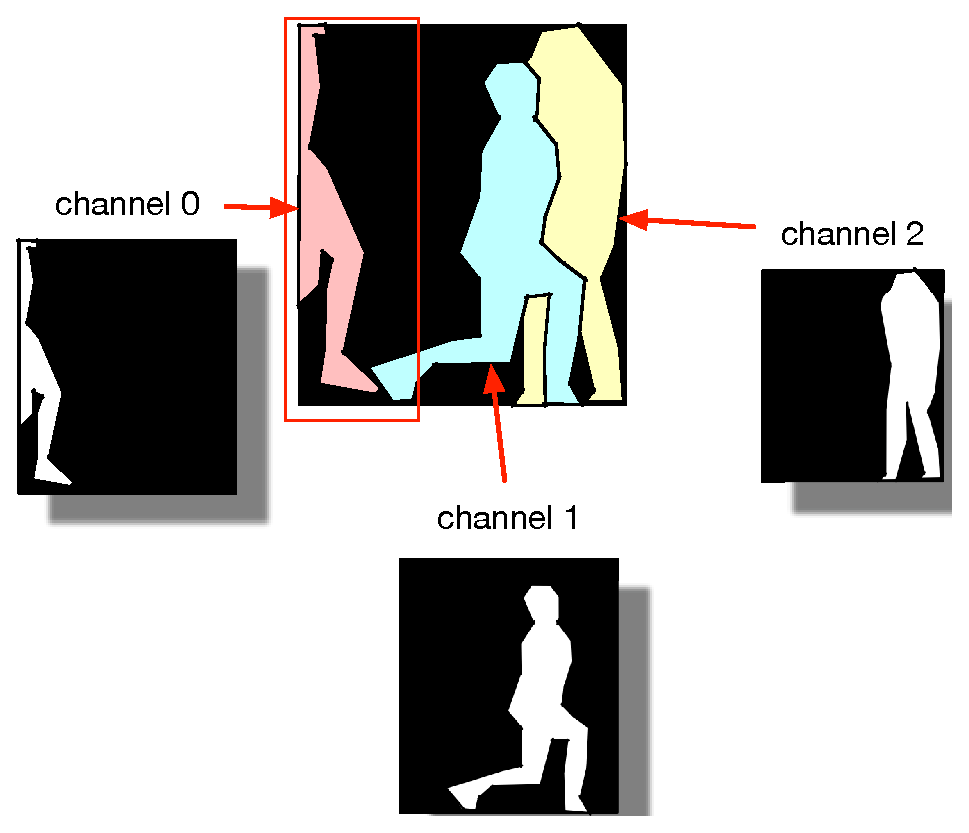
\includegraphics[scale=0.34]{instance_segmentation.eps}
	\caption{Channel-wise instance segmentation}
	\label{fig:chInsSeg}
\end{figure}

\section{本章小结}
